\documentclass[11pt,letterpaper]{article}
\usepackage{listings}
\usepackage{graphicx}
\lstset{basicstyle=\small\ttfamily}
\begin{document}
\title {A Tutorial on the Adele Programming Language}
\author {
	Jen-Chieh Huang \texttt{(jh3478)} \and Xiuhan Hu \texttt{(xh2234)} \and     
	Zixuan Gong \texttt{(zg2203)} \and Jie-Gang Kuang \texttt{(jk3735)} \and 
	Yuan Lin \texttt{(ly2324)}
}
\maketitle
\pagebreak
%%%%%%%%%%%%%%%%%%%%%%%%%%%%%%%%%%%%%%%%%%%%%%%%%%%%%
\section {Introduction}

ASCII-art description language, Adele, is a domain-specific programming language aimed at providing a simple and intuitive way to describe and generate ASCII artworks. It includes several special language constructs for ASCII artwork. Besides, common programming language features such as functions, control statements are also supported. Adele is also designed to be executed in a portable run-time environment. The final executable of an Adele program can be run in any web browser supporting JavaScript. 

Before discussing the details of the language, we'd like to present the basic concepts of how Adele processes the output ASCII art. For every Adele program, a canvas is given to the main function. The canvas is the destination on which a user can put his artwork on. When a user puts something on the artwork, it generates a corresponding 'layer' on the canvas. This is exceptionally useful when the user would like to create reusable parts and background parts of the artwork. The user can change the position of the reusable parts to create interactive or animated effects. When all the layers are created, the user would need to inform the run-time environment, and the resulting canvas will be displayed on the output device.

The purpose of the document is to show the audience how to write and execute an Adele program. The document will first start by giving a simple example of an Adele program and how to run this program followed by more complicated examples and details of the special constructs. Finally, we will present an example by putting everything together.

Good luck and have fun in Adele.

\section {The First Adele Program}

As a tradition in introducing a programming language, we would like to present the Hello World as our first example using Adele. The following codes illustrate what the Hello World program looks like.

\lstinputlisting[frame=single] {./hello_world.adele}

In the program, the entry point of any Adele program is the main function. 'void' indicates that the return value of the function is ignored, and the parenthesis after the function name shows the parameters of the function. In this example, c, whose type is canvas, is the input parameter to the main function, which is the output device of the user's artwork. For user-defined function, empty parameters are also possible. Note that, in Adele, every function has to be ended with an 'end' marker.

In the 2nd line, the function, print\_str, is a predefined function which takes 3 parameters. The first 2 parameters are the x and y coordinator in the default canvas, and the 3rd parameter is the string which the user would like to show. The semantics of the function is that the a ASCII-string will be displayed on the user window at the given location.

After compilation and execution, you should be able to see the string printed on the screen at the upper left corner. The details of the compilation and execution is listed in the following section.

%%%%%%%%%%%%%%%%%%%%%%%%%%%%%%%%%%%%%%%%%%%%%%%%%%%%%
\section {Compiling and Running}
To use our compiler, you need to create your program file whose name ends in ".adele"(other suffix is never recommended), such as "test.adele". Then you can compile it by the following command:

\begin{lstlisting}[tabsize=4]
	adelecc test.adele -o test.html
\end{lstlisting}

where test.html is the output file. Note that our compiler is actually a java class file, a java runtime environment is required(8.0 or later).

If you make everything correct, including any spelling and grammar, our compile will produce the file test.html as you want with no warning or error. Then you can open it with any text editor to view or modify its content(But it may be a struggle to understand, so modification is never recommended). Or you can just open it using your favorite browser to see your fancy arts created via our language.

About the runtime environment, as stated before, all you need is a java runtime environment. So don't worry too much about your system. Maybe you can enjoy the joy of creating cool ascii-arts just on your phone.

%%%%%%%%%%%%%%%%%%%%%%%%%%%%%%%%%%%%%%%%%%%%%%%%%%%%%
\section {More Complex Examples}

In Adele, there are some control flow statements and user defined structures to help you write less code.

\subsection {if conditional statements}

The if statement allows you to control if a program enters a block of code based on whether a given condition is true. For example:

\begin{lstlisting}[caption=if.adl, label=if, captionpos=b, tabsize=4, frame=single]
x = 1;
if (x==1)
	print_str (0, 0, "x is equal to 1");
end

if (x==2)
	print_str (0, 0, "x is equal to 2");
end
# "x is equal to 1" is printed
\end{lstlisting}

All if statements end with a keyword end.

\subsection {while loop statements}

The while statement loops through a block of code as long as a specified condition is true. For instance:

\begin{lstlisting}[caption=while.adl, label=while, captionpos=b, tabsize=4, frame=single]
x = 1;
sum = 0;

while (x<=100)
  sum = sum + x;
  x = x + 1;
end
# x = 51, sum = 5050
\end{lstlisting}

Again, while loops end with keyword end. Actually, a rule of thumb for Adele is that all control flow statements end the block of code with an end marker.

\subsection {functions}
A function is a group of statements that is given a name, and which can be called from some point of the program. The common syntax to define a function is:

\begin{lstlisting}
type name(parameter1, parameter2, ...)
statement1
statement2
...
end
\end{lstlisting}

For example, here is a complete Adele program:

\begin{lstlisting}[caption=func.adl, label=func, captionpos=b, tabsize=4, frame=single]
int isGreaterThanZero (int x)
  if (x>0)
    return 1;
  end
  return 0;
end

void main(canvas c)
  int t = 10;
  t = isGreaterThanZero(t); # t = 1
end
\end{lstlisting}

The main function is required for any Adele program. Besides the main function, we defined another function named isGreaterThanZero. We should not define a function inside another, which means nested functions are not allowed.

To call a function, use name(parameter1, parameter2, ...) to fill in any expression. We can recursively call a function if needed.

\subsection {User-defined group structures}
Sometimes we may want to group a list of variables under a same name by defining a group structure. Here is an example:

\begin{lstlisting}
group point
  int x;
  int y;
end
\end{lstlisting}

To declare an instance variable of a specific group point:
\begin{lstlisting}
group point p1;
\end{lstlisting}

To access a member of a group instance, we use the conventional dot (.) operator:
\begin{lstlisting}
p1.x = 10;
p1.y = 20;
\end{lstlisting}

Group variables are passing by reference in expression evaluation, which is different from primitive-typed variables.

\subsection {Example: Sorting using Adele}

Here is an implementation of quick sort algorithm in Adele language:

\begin{lstlisting}[caption=qsort.adl, label=qsort, captionpos=b, frame=single, tabsize=4]
void qsort (int A[], int left, int right)
	int i = left;
	int j = right;
	int tmp;
	int pivot = A[0];

	while (i<=j)
		while (A[i]<pivot)
			i = i + 1;
		end
  		
		while (A[j]>pivot)
			j = j - 1;
		end
  		
  		if (i<=j)
			tmp = A[i];
			A[i] = A[j];
			A[j] = tmp;
			i = i + 1;
			j = j - 1;
		end
	end

	if (left < j)
  		qsort (A, left, j)
	end

	if (right > i)
  		qsort (A, i, right)
	end
end
\end{lstlisting}


%%%%%%%%%%%%%%%%%%%%%%%%%%%%%%%%%%%%%%%%%%%%%%%%%%%%%
\section {Special Constructs}

Function print(x, y, graph) is used to put a graph on the canvas at a position relative to it. But sometimes users may want to place a graph relative to another graph, rather than the canvas. The following special constructs provided by Adele are introduced for this purpose. More precisely speaking, these constructs offer different ways to combine two graphs into a new graph.

\subsection {Overlay and locate}

The overlay symbol ‘//’ is used together with the locate symbol ‘\@’, and the two symbols form a ternary operator. The syntax of the construct is:

\begin{lstlisting}
    graph_a // graph_b @ (pos_x, pos_y);
\end{lstlisting}

The first two parameters are graphs, and the two parameters inside the parentheses are integers, which can be negative. The effect of this construct is that graph\_a overlays graph\_b, and the upper left corner of graph\_a is placed at the position (pos\_x, pos\_y) relative to the upper left corner of graph\_b. The return value of the construct is a graph. Consider the following example:

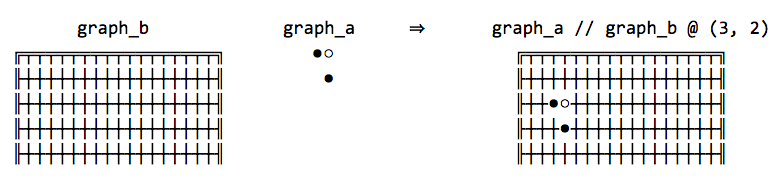
\includegraphics[width=\textwidth]{./graph_01.png}

It's clear that the graph on the left side of the overlay symbol is in the upper layer; the one on the right side is in the lower layer. Notice that graph\_a and graph\_b stay unchanged after applying the operator. And as shown in the above example, the cells of the upper layer that are white spaces would not replace the corresponding cells of the lower layer.

\subsection {Attach Horizontally/Vertically}

To attach a graph to the border of another graph, users can use the overlay and locate construct, and specify the exact coordinate of a cell on that border. Adele provides two utility constructs to facilitate that operation.

To attach graph\_a to the right of graph\_b (i.e. attach horizontally):
\begin{lstlisting}
    graph_b - graph_a
\end{lstlisting}

To attach graph\_a to the bottom of graph\_b (i.e. attach vertically):
\begin{lstlisting}
    graph_b | graph_a
\end{lstlisting}

The parameter on the left side of the operator is the "base" graph, and the one on the right side is the graph to attach to it. As the overlay and locate operator, applying the two operators ('-' or '|') does not change the value of the two graphs, and each construct returns a new graph. Consider the following example:

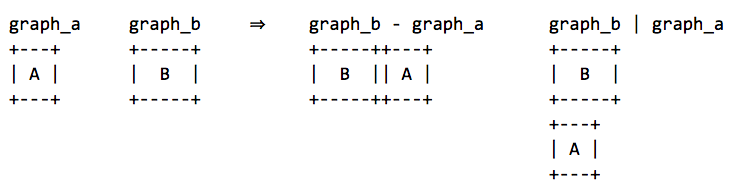
\includegraphics[width=\textwidth]{./graph_02.png}

The example shows that, the "attach horizontally" operator sets the top-left corner of graph\_a to the right of the top-right corner of graph\_b; the "attach vertically" operator sets the top-left corner of graph\_a to the bottom of the bottom-left corner of graph\_b. Therefore, if users want to customize the position of graph\_a, relative to the border of the graph\_b, it's still suggested to use the overlay and locate construct. For example, to realize the following effect:

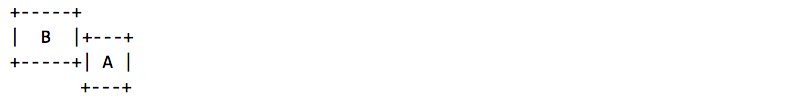
\includegraphics[width=\textwidth]{./graph_03.png}

%%%%%%%%%%%%%%%%%%%%%%%%%%%%%%%%%%%%%%%%%%%%%%%%%%%%%
\section {Predefined Functions}

Besides the data types and flow control, some more utilities are provided either to enable display or to facilitate programming process.

\subsection {draw}
The draw function is the essential function to display the ASCII art arranged by the programmers. All the graph data defined or placed in the program is not displayed immediately. Adele will trigger the target language to render the output only when the draw function is invoked. The usage of draw is
\begin{lstlisting}[tabsize=4] 
	draw (); 
\end{lstlisting}
and it does not return any value. Here is a simple example to show the usage of the draw function.

\begin{lstlisting}[tabsize=4, frame=single]
void main (canvas c)
	graph g = “\(^o^)/”;
	g@(0, 0);
	draw();
end
\end{lstlisting}

In the example, if the program ends without draw(), the output will actually not render the graph. Only with draw() will the Adele generate the rendering part of target code to show the graphs.

The purpose of this step is mainly to coordinate and synchronize the display timing of different graphs. When there are two or more graphs to be displayed at the same time, we can hardly achieve it without draw(). If there is no draw(), and we display the graph immediately when we put the graph on the canvas by g\@(0, 0). For more graphs operated with this mechanism, those graphs will be displayed one by one but not at the same time.

\subsection {print}
In addition to the ASCII art, sometimes the programmers would like to add some words in the picture for various reasons. Adele provides a simple function for such a situation. The usage of the string printing function is
\begin{lstlisting}[tabsize=4]
	print_str(<x>, <y>, "<string>");
\end{lstlisting}
and it does not return values.

Since this is just a simple and quick implementation to display strings, there are two restrictions when using this function. One is that, although the displayed strings are treated as a graph, the lifetime of the graph is only to the next draw function. After the string is rendered by a draw(), it will not be displayed again in the next draw() unless the same statement is invoked again before the draw(). This is because there is no reference to the string(graph) so that we cannot remove it manually with statements.

The other is that the rendered string will always on the most bottom layer. The reason is similar to the previous one. Since we do not have a reference to the string, we cannot decide the layer of it, or place it over or under other graphs. As a result, in order not to affect the major part of the graphs, all the strings rendered by the string printing function will be under all other explicit graph types.

\subsection {load}
It is most of the case that the elemental ASCII graphs are preferably constructed from the existing files rather than locally with the character arrays in the programs. For these cases, a predefined function, load, can be used to import ASCII graphs from the files. The usage of load is
\begin{lstlisting}[tabsize=4]
	load("filename");
\end{lstlisting}
and it returns a graph-type reference which points to a ASCII character group.

For example, to show a ASCII graph of $\backslash$ (\^o\^)/ without the file importing, a simple program as in section 6.1 is
\begin{lstlisting}[caption=hail.adl, label=hail, captionpos=b, tabsize=4, frame=single]
void main()
	graph g = "\(^o^)/";
	g@(0, 0);
	draw();
end
\end{lstlisting}

Alternatively, It can also be done by having a text file of $\backslash$ (\^o\^)/ and a program to import the graph from the file, such as

\begin{lstlisting}[caption=graph.txt, label=hail_face, captionpos=b, tabsize=4]
						\(^o^)/
\end{lstlisting}

\begin{lstlisting}[caption=hailv2.adl, label=hailv2, captionpos=b, tabsize=4, frame=single]
void main()
	graph g = load ("graph.txt");
	draw();
end
\end{lstlisting}

Although the above example may be too simple to show the convenience of using load to import the graphs from the files, the load function can be very useful when there are multiple rather bigger graphs to manipulate. The following program is an example to demonstrate the advantage of using the load function
\pagebreak
\begin{lstlisting}[caption=graph\_horse.txt, label=horse, captionpos=b]
		   >>\.
		  /_  )`.
		 /  _)`^)`.   _.---. _
		(_,' \  `^-)""      `.\
		      |              | \
		      \              / |
		     / \  /.___.'\  (\ (_
		    < ,"||     \ |`. \`-'
		     \\ ()      )|  )/
		     |_>|>     /_] //
		       /_]        /_]
\end{lstlisting}

\begin{lstlisting}[caption=graph\_cat.txt, label=cat, captionpos=b]
			  A_A
			 (-.-)
			  |-|
			 /   \
			|     |   __
			|  || |  |  \__
			 \_||_/_/
\end{lstlisting}

\begin{lstlisting}[caption=graph\_dogs.txt, label=dogs, captionpos=b]
_     /)---(\          /~~~\
\\   (/ . . \)        /  .. \
 \\__)-\(*)/         (_,\  |_)
 \_       (_         /   \@/    /^^^\
 (___/-(____) _     /      \   / . . \
              \\   /  `    |   V\ Y /V
               \\/  \   | _\    / - \
                \   /__'|| \\_  |    \
                 \_____)|_).\_).||(__V
\end{lstlisting}

\begin{lstlisting}[caption=animals.adl, label=animal, captionpos=b, tabsize=4, frame=single]
void main()
	graph gHorse = load ("graph_horse.txt");
	graph gCat = load ("graph_cat.txt");
	graph gDogs = load("graph_dogs.txt");
	print(0, 0, gHorse);
	print(25, 25, gCat);
	print(30, 0, gDogs);
	draw();
end
\end{lstlisting}

However, there are some restrictions or things to be aware of when using the load function. First of all, the source file should be ASCII-encoded text file. The result of opening a non-ASCII text file is unpredictable. Second, the content of a single text file will be grouped as one graph. There is no way for the load function to load partial graph in the source file.

\subsection {sleep}

Despite the basic flow control described in the previous chapter, a time control mechanism is necessary to generate the animation. Therefore, Adele provides the sleep function to pause the procedure in the program to enable the graphs to be displayed step by step. The usage of the sleep function is
\begin{lstlisting}[tabsize=4]
	sleep (time_in_milliseconds);
\end{lstlisting}
and it does not return values.

An example program to show the usage of the sleep function is like

\begin{lstlisting}[caption=marquee.adl, label=marquee, captionpos=b, , tabsize=4, frame=single]
void main ()
	graph g = "This is a scrolling text";
	int x = 0;
	int y = 0;
		
	while (true)
		g@(x, y);
		draw();
		sleep(100);
		x = x + 1;
		if (x == 80)
			x = 0;
		end
	end
end
\end{lstlisting}

%%%%%%%%%%%%%%%%%%%%%%%%%%%%%%%%%%%%%%%%%%%%%%%%%%%%%
\section {Put Everything Altogether}

\end{document}

